\documentclass[pdflatex,sn-mathphys-num,iicol]{sn-jnl}

\usepackage[T1]{fontenc}
\usepackage{amsmath,amssymb}
\usepackage{float}
\floatstyle{ruled}
\newfloat{algorithm}{tbp}{loa}
\floatname{algorithm}{Algorithm}
\usepackage{algpseudocode}
\usepackage{booktabs}
\usepackage{graphicx}
\usepackage{tabularx}
\usepackage{tikz}
\usepackage{pgfplots}
\pgfplotsset{compat=1.17}
\usepgfplotslibrary{groupplots}
\usetikzlibrary{arrows.meta,calc,positioning}
\hypersetup{hypertexnames=false}

\raggedbottom
\setcounter{dbltopnumber}{2}

\begin{document}

\title[AC-MOT]{AC-MOT: Optimization-Guided Adaptive Detector Operating-Point Control for Aerial Multi-Object Tracking}

\author*[1]{\fnm{Ahmed Gouda} \sur{Ismail}}\email{a7medgouda1@gmail.com}
\author[1]{\fnm{Mohamed S.} \sur{Mohamed}}\email{mohamedms@mtc.edu.eg}
\author[2]{\fnm{Tarek Ahmed} \sur{Mahmoud}}\email{tarek.mohamed@eui.edu.eg}

\affil*[1]{\orgdiv{Computer Engineering and Artificial Intelligence Department}, \orgname{Military Technical College}, \orgaddress{\city{Cairo}, \country{Egypt}}}
\affil[2]{\orgdiv{Computer Engineering Department}, \orgname{Egypt University of Informatics}, \orgaddress{\city{Cairo}, \country{Egypt}}}

\abstract{Multi-object tracking (MOT) in unmanned aerial vehicle (UAV) videos is challenging due to variations in object density, size, illumination, and blur. However, most tracking-by-detection systems use fixed detector settings that may not suit changing scene conditions. This paper proposes Adaptive Control for Multi-Object Tracking (AC-MOT), a training-free framework that dynamically adjusts the detector operating point, defined by the confidence threshold, non-maximum suppression (NMS) intersection-over-union (IoU) threshold, and input resolution. Using only the current frame and past tracking information, AC-MOT treats the detector operating point as an online control variable without modifying or retraining the detector or tracker. Initial optimization experiments reveal trade-offs among tracking accuracy, identity preservation, and computational efficiency, motivating a three-state controller. On VisDrone, AC-MOT improves Higher Order Tracking Accuracy (HOTA) from 41.586 to 44.523, Multiple Object Tracking Accuracy (MOTA) from 9.876 to 27.871, and Identity F1 Score (IDF1) from 48.569 to 53.929 with ByteTrack, while reducing identity switches (IDS) from 1,341 to 1,016. With OATrack, MOTA increases from 28.165 to 34.483, and IDS decreases from 773 to 604. Paired bootstrap analysis with 5,000 resamples supports improvements in HOTA, MOTA, IDF1, and IDS for both trackers. Cross-dataset evaluation on UAVDT, using the same fixed policy without retuning, improves MOTA by 17.601 and 3.267 points with ByteTrack and OATrack, respectively. These results demonstrate that online detector operating-point adaptation can improve aerial MOT performance with limited computational overhead and no additional training.}

\keywords{multi-object tracking, UAV video, adaptive inference, detector operating point, real-time image processing}

\maketitle

\section{Introduction}\label{sec:intro}

Unmanned aerial vehicles (UAVs) are widely used for traffic monitoring,
surveillance, and search, and many of these tasks need multi-object tracking
(MOT): every object must be detected in every frame and keep the same
identity over time \cite{wu2022uavsurvey,zhu2022visdrone}. Aerial video makes
this hard. Objects are small, their number changes quickly, the camera moves,
and illumination and blur change within one video
\cite{zhu2022visdrone,du2018uavdt,cheng2023smallobject}. Many of these
applications also need results with low delay, so the processing cost matters
as much as the accuracy.

The performance of aerial multi-object tracking depends on several factors, including the quality of object detection, the ability to associate objects across consecutive frames, and the computational resources available for processing. These factors are closely related, since errors in object detection can directly affect the tracking process. Missed detections may interrupt object trajectories, while false detections can lead to incorrect associations and identity switches. At the same time, improving detection accuracy often requires additional computation, which may increase processing time and limit real-time performance. Achieving a suitable balance between detection quality, tracking accuracy, identity consistency, and computational efficiency is therefore an important challenge in aerial MOT systems.

Most MOT systems follow the tracking-by-detection design. A detector finds the
objects in each frame, and a tracker links the detections over time
\cite{bewley2016sort,zhang2022bytetrack}. Much research improves the tracker,
for example its motion model or its association rules, and much research
improves the detector itself. Far less attention is given to how the detector
is run. In practice the detector uses one confidence threshold, one
non-maximum-suppression (NMS) threshold, and one input resolution for the
whole video. These three values form the detector operating point, and they
decide which boxes reach the tracker.

A fixed operating point does not fit a scene that keeps changing. A setting
that works in a sparse, clear scene can keep too much clutter in a dense
scene. A setting that works in a dense scene can lose small or weak objects in
another part of the same video. A large input helps small objects, but it
costs the same time on easy and hard frames. The choice therefore moves false
positives, missed objects, identity switches, and runtime together.

Existing adaptive methods only partly address this problem. Adaptive inference
methods change the detector's input scale or configuration, but they usually
need an extra learned model and are designed for detection, not tracking
\cite{chin2019adascale,xu2020approxdet}. Adaptive tracking methods change
thresholds inside one specific tracker \cite{ma2023adaptivebytetrack,shim2024adaptrack}.
What is missing is a simple, training-free way to adapt the detector
operating point online for MOT, without changing the detector or the tracker.

This paper presents AC-MOT, a training-free control layer that adapts the
detector operating point online for aerial MOT. It sits between the detector
and the tracker, reads inexpensive scene cues, and works with existing
detectors and trackers without retraining or modifying them. The method is
described in Sect.~\ref{sec:method}, and Sect.~\ref{sec:development} explains
how it was developed with optimization and tested step by step.

The main contributions are:
\begin{enumerate}
\item A training-free control layer that treats the detector operating point
      as part of the MOT system and adapts it online (Sect.~\ref{sec:method}).
\item An optimization-guided development path, in which each step is compared
      with the baseline it was built on (Sect.~\ref{sec:development}).
\item An evaluation on VisDrone2019-MOT with two trackers, ByteTrack and the
      recent OATrack, using eight MOT metrics and paired bootstrap intervals,
      together with a transfer to UAVDT without retuning
      (Sect.~\ref{sec:results}).
\item A latency measurement showing that the control layer adds only a few
      milliseconds per frame on a Tesla T4 GPU (Sect.~\ref{sec:discussion}).
\end{enumerate}

The rest of the paper is organized as follows. Section~\ref{sec:related}
describes the datasets and evaluation metrics and reviews related work. Section~\ref{sec:method} describes AC-MOT, and
Section~\ref{sec:development} explains how it was developed.
Section~\ref{sec:results} gives the experimental settings and the results,
and Section~\ref{sec:discussion} a discussion. Section~\ref{sec:conclusion} concludes the paper.
\section{Background and Related Work}\label{sec:related}
This section first describes the datasets and the evaluation metrics used in
this paper and then reviews related work on multi-object tracking.

\subsection{Dataset Description}\label{sec:datasets}
\emph{VisDrone.} VisDrone \cite{zhu2022visdrone} is a large-scale benchmark
recorded by various drone-mounted cameras in 14 cities in China. It covers
urban and rural regions and both sparse and crowded scenes. It consists of 263
video clips with 179,264 frames and 10,209 static images, in which more than
2.5 million boxes of 10 object categories are annotated. The static images form
the image detection track (VisDrone-DET), with 6,471 training, 548
validation, 1,580 test-challenge, and 1,610 test-dev images. The
multi-object tracking track (VisDrone-MOT) uses 96 video clips: 56 for
training (24,198 frames), 7 for validation (2,846 frames), 16 for challenge
testing (6,322 frames), and 17 for development testing (6,635 frames). It
evaluates five categories: pedestrian, car, van, bus, and truck
\cite{zhu2022visdrone}. In this paper, eight training clips serve as
calibration data for the final controller (Sect.~\ref{sec:modern}), and the
seven validation clips serve as evaluation data (Sect.~\ref{sec:results}).

\emph{UAVDT.} UAVDT \cite{du2018uavdt} consists of 100 video sequences
selected from more than 10 hours of video taken with a UAV platform at
locations in urban areas, including squares, arterial streets, toll stations,
highways, crossings, and T-junctions. The videos are recorded at 30 frames per
second with a resolution of $1080\times540$ pixels. About 80,000 frames are
annotated with 0.84 million boxes of more than 2,700 vehicles in three
categories (car, truck, and bus), together with attributes such as weather
condition, flying altitude, and camera view. The test set contains 20
sequences for the detection and multi-object tracking tasks
\cite{du2018uavdt}. This paper uses these 20 test sequences to test the
transfer of AC-MOT without retuning (Sect.~\ref{sec:results}).

\subsection{Multi-Object Tracking Evaluation Metrics}\label{sec:metrics}
This paper reports HOTA, MOTA, IDF1, IDS, FP, FN, precision, and recall. They
are defined as follows \cite{dendorfer2021motchallenge,luiten2021hota}.

\emph{Detection errors.} In each frame $t$, output boxes are matched one to
one to ground-truth boxes with an IoU of at least 0.5. Let $\mathrm{GT}_t$ be
the number of ground-truth boxes, $\mathrm{TP}_t$ the number of matched pairs,
$\mathrm{FP}_t$ the number of output boxes without a match (false positives),
and $\mathrm{FN}_t$ the number of ground-truth boxes without a match (false
negatives, or missed objects). Over all frames,
\begin{align}
\mathrm{GT}&=\sum_t \mathrm{GT}_t,\qquad \mathrm{TP}=\sum_t \mathrm{TP}_t,\label{eq:gt}\\
\mathrm{FP}&=\sum_t \mathrm{FP}_t,\qquad \mathrm{FN}=\sum_t \mathrm{FN}_t,\label{eq:fpfn}
\end{align}
so that $\mathrm{TP}=\mathrm{GT}-\mathrm{FN}$. Precision is the fraction of
output boxes that are correct, and recall is the fraction of ground-truth
boxes that are found:
\begin{equation}
\mathrm{Precision}=\frac{\mathrm{TP}}{\mathrm{TP}+\mathrm{FP}},\qquad
\mathrm{Recall}=\frac{\mathrm{TP}}{\mathrm{GT}}.
\label{eq:prrc}
\end{equation}

\emph{Identity switches.} Let $\phi_t(i)$ be the output track matched to
ground-truth object $i$ in frame $t$, and $\phi_{\mathrm{prev}}(i)$ the
output track to which object $i$ was last matched before $t$. An identity
switch is counted whenever these two tracks differ:
\begin{equation}
\mathrm{IDS}=\sum_t\sum_{i}\mathbf{1}\!\left[\phi_t(i)\neq\phi_{\mathrm{prev}}(i)\right],
\label{eq:ids}
\end{equation}
where the inner sum runs over the objects that are matched in frame $t$ and
were matched before.

\emph{MOTA and IDF1.} MOTA combines the three error types, and IDF1 measures
how long each object keeps the correct identity:
\begin{align}
\mathrm{MOTA}&=1-\frac{\mathrm{FN}+\mathrm{FP}+\mathrm{IDS}}{\mathrm{GT}},\label{eq:mota}\\
\mathrm{IDF1}&=\frac{2\,\mathrm{IDTP}}{2\,\mathrm{IDTP}+\mathrm{IDFP}+\mathrm{IDFN}}.\label{eq:idf1}
\end{align}
For IDF1, each ground-truth track is first matched to at most one output
track over the whole video. IDTP, IDFP, and IDFN are then the true-positive,
false-positive, and false-negative boxes under this track-level matching.

\emph{HOTA.} HOTA balances detection and association \cite{luiten2021hota}.
At a localization threshold $\alpha$, let $\mathrm{TP}_\alpha$,
$\mathrm{FN}_\alpha$, and $\mathrm{FP}_\alpha$ be the matched pairs, missed
ground-truth boxes, and unmatched output boxes. For a matched pair $c$,
$\mathrm{TPA}(c)$ is the set of matched pairs with the same ground-truth
identity and the same output identity as $c$; $\mathrm{FNA}(c)$ is the set of
boxes of the same ground-truth object that are matched to another output
identity or not matched; and $\mathrm{FPA}(c)$ is the set of boxes of the same
output track that are matched to another object or not matched. Then
\begin{align}
\mathrm{DetA}_\alpha&=\frac{|\mathrm{TP}_\alpha|}{|\mathrm{TP}_\alpha|+|\mathrm{FN}_\alpha|+|\mathrm{FP}_\alpha|},\label{eq:deta}\\
\mathcal{A}(c)&=\frac{|\mathrm{TPA}(c)|}{|\mathrm{TPA}(c)|+|\mathrm{FNA}(c)|+|\mathrm{FPA}(c)|},\label{eq:ac}\\
\mathrm{AssA}_\alpha&=\frac{1}{|\mathrm{TP}_\alpha|}\sum_{c\in\mathrm{TP}_\alpha}\mathcal{A}(c),\label{eq:assa}\\
\mathrm{HOTA}&=\frac{1}{19}\sum_{\alpha}\sqrt{\mathrm{DetA}_\alpha\,\mathrm{AssA}_\alpha},\label{eq:hota}
\end{align}
where $\alpha$ runs over $0.05, 0.10, \dots, 0.95$. All scores except the
counts IDS, FP, and FN are given in percent.

Paired bootstrap resampling at the sequence level keeps the dependence within
each sequence and gives intervals for system differences
\cite{efron1993bootstrap}. Each resample draws the evaluation sequences with
replacement. The same draw is used for both systems, the pooled metrics are
recomputed, and their difference is recorded. The 95\% interval is the
2.5--97.5 percentile range.

\subsection{Multi-Object Tracking Literature Survey}
Multi-object tracking has been widely studied, with research focusing on improving object detection, data association, and tracking accuracy under different operating conditions. In aerial videos, these tasks become more challenging because of small objects, camera motion, and frequent changes in scene characteristics. Previous studies have addressed these challenges through improved tracking algorithms, adaptive threshold selection, and dynamic inference techniques. In addition, optimization methods and performance evaluation measures have been used to investigate the trade-offs between tracking accuracy and computational efficiency. This section reviews these research directions and discusses their relevance to the problem addressed in this paper.

\subsubsection{Tracking-by-Detection Methods in Aerial MOT}\label{sec:hosts}
Tracking-by-detection is one of the most widely used approaches in multi-object tracking (MOT). In this framework, objects are detected in individual video frames and then associated across consecutive frames to maintain their identities. Several methods have been developed to improve detection reliability, motion prediction, and data association. However, tracking objects in aerial videos introduces additional challenges that require specialized detection and tracking techniques.

SORT built a compact online pipeline from motion prediction and assignment
\cite{bewley2016sort}, and StrongSORT adds appearance features to reduce
identity fragmentation \cite{du2023strongsort}. ByteTrack first associates
high-confidence detections and then uses low-confidence boxes to recover
objects that would otherwise be lost \cite{zhang2022bytetrack}. TrackFormer
performs detection and association with transformer queries
\cite{meinhardt2022trackformer}. Standard evaluation follows the MOTChallenge
benchmarks \cite{dendorfer2021motchallenge}.

Aerial video adds small targets, changing object counts, camera motion, and
clutter \cite{zhu2022visdrone,du2018uavdt}. UAVMOT addresses the motion of the
UAV camera inside the tracker \cite{liu2022uavmot}, and LSO-YOLO designs a
lightweight real-time detector for small UAV objects \cite{dai2026lsoyolo}.
OATrack \cite{qi2026oatrack} is a recent UAV small-object tracker published in
2026. It weights association by detection quality and uses a YOLO detection
cache. We use OATrack as a second host and keep it unchanged. With the same
detector, AC-MOT improves its results in our pipeline: HOTA rises by 1.325,
MOTA by 6.318, and IDF1 by 2.258 points, and IDS fall by 169
(Sect.~\ref{sec:results}). These works improve the tracker or the detector
itself. AC-MOT asks a different question: which detector setting should be
used for the current scene.

\emph{Detector and trackers used in this study.} The experiments use the YOLO11m detector \cite{jocher2024yolo11}, a
one-stage detector of the Ultralytics YOLO family, in a public version trained
on the VisDrone2019-DET dataset \cite{zhu2022visdrone}. Two of the trackers
above serve as hosts. ByteTrack \cite{zhang2022bytetrack} is a widely used
tracker whose second association step uses low-score boxes. OATrack
\cite{qi2026oatrack} is a recent tracker for small UAV objects that weights
association by detection quality. Both hosts are used without modification.

\subsubsection{Adaptive Threshold Selection in Multi-Object Tracking}
Several studies have investigated adaptive threshold selection to improve multi-object tracking under changing scene conditions. In conventional tracking-by-detection systems, fixed thresholds are commonly used to determine which detections are accepted and how they are associated with existing tracks. However, the reliability of these thresholds may vary when object density, occlusion, and detection confidence change during a video sequence. Adaptive threshold methods attempt to address this limitation by adjusting selected tracking parameters according to the current conditions.

Adaptive ByteTrack adjusts the confidence threshold used within the ByteTrack \cite{ma2023adaptivebytetrack} algorithm to accommodate variations in detection confidence. This can help the tracker handle objects whose detection scores change because of occlusion, small object size, or changes in image quality. Similarly, AdapTrack \cite{shim2024adaptrack} adapts the matching thresholds used during data association. By adjusting these thresholds, the tracker can modify its association decisions according to the available detection and tracking information. Although both approaches introduce flexibility into the tracking process, their adaptation mechanisms operate within the tracker and are designed around particular tracking algorithms.

AC-MOT follows a different approach by adapting the detector operating point rather than the internal parameters of the tracker. The detector operating point consists of three parameters: the detection confidence threshold, the non-maximum suppression (NMS) intersection-over-union (IoU) threshold, and the input resolution. Each parameter influences the detections passed to the tracker. The confidence threshold determines which low-confidence detections are retained, the NMS threshold controls the suppression of overlapping bounding boxes, and the input resolution affects the visibility of small objects and the computational cost of detection. Adjusting these parameters together allows the detector configuration to respond to changes in scene conditions before the tracking stage.

An important distinction is that AC-MOT does not require changes to the tracking algorithm. Instead, it operates as an external control mechanism that selects detector configurations using scene information and previous tracking results. The selected configuration is then applied during detector inference, while the tracker continues to perform its original association and identity management procedures. This design allows AC-MOT to be evaluated with different trackers, including ByteTrack and OATrack, without modifying or retraining either tracker. Therefore, AC-MOT extends adaptive parameter selection beyond tracker-specific thresholds by introducing joint detector operating-point control within the overall MOT pipeline.

\subsubsection{Adaptive Inference for Object Detection}
Dynamic neural networks change their structure or parameters for each input
\cite{han2022dynamic}, and resolution-adaptive networks spend less computation
on easy inputs \cite{yang2020ranet}. AdaScale selects the input scale of each
video frame with a scale regressor trained on detector features
\cite{chin2019adascale}. ApproxDet switches detection configurations at run
time with accuracy and latency models trained offline \cite{xu2020approxdet}.
Chameleon re-profiles the configuration of video analytics pipelines over time
\cite{jiang2018chameleon}. These adaptive inference methods mainly aim to improve object detection accuracy, reduce computational cost, or achieve a suitable balance between accuracy and processing time. To select appropriate inference configurations, some approaches rely on additional trained models, such as scale predictors or offline accuracy and latency estimators, while others use periodic profiling to respond to changes in video content. However, their adaptation strategies are generally designed for object detection or video analytics rather than the specific requirements of multi-object tracking, where detection errors can also affect object association and identity consistency. In contrast, AC-MOT focuses on improving tracking performance by dynamically adjusting three detector parameters: the confidence threshold, non-maximum suppression (NMS) IoU threshold, and input resolution. Its controller uses lightweight scene information and previous tracking results to select detector configurations without requiring an additional learned model or retraining the existing detector or tracker. Furthermore, AC-MOT is evaluated using tracking-specific metrics, including tracking accuracy, identity preservation, and association quality, with two different tracking algorithms, ByteTrack and OATrack. Table~\ref{tab:related} summarizes the main differences between AC-MOT and the existing adaptive inference approaches.

\begin{table}[t]
\caption{Adaptive methods closest to AC-MOT (BT: ByteTrack).}
\label{tab:related}
\centering\footnotesize
\setlength{\tabcolsep}{3pt}
\begin{tabular}{@{}l>{\raggedright\arraybackslash}p{20mm}>{\raggedright\arraybackslash}p{17mm}>{\raggedright\arraybackslash}p{13mm}@{}}
\toprule
Method & Adapted & Where & Task\\
\midrule
AdaScale \cite{chin2019adascale} & input scale & detector & video detection\\
ApproxDet \cite{xu2020approxdet} & detection configuration & detector & video detection\\
Chameleon \cite{jiang2018chameleon} & pipeline configuration & analytics pipeline & video analytics\\
Adapt.\ BT \cite{ma2023adaptivebytetrack} & confidence threshold & inside BT & MOT\\
AdapTrack \cite{shim2024adaptrack} & matching thresholds & inside the tracker & MOT\\
AC-MOT & confidence, NMS, resolution & detector; tracker unchanged & aerial MOT\\
\bottomrule
\end{tabular}
\end{table}

\subsubsection{Optimization and Evaluation for Multi-Object Tracking}
Optimization and performance evaluation play an important role in developing reliable multi-object tracking (MOT) systems. The selection of detector and tracking parameters can affect detection accuracy, object association, identity consistency, and computational efficiency. Since improving one aspect of tracking performance may negatively affect another, systematic optimization methods are needed to explore different parameter configurations and identify suitable trade-offs. In addition, evaluating tracking systems requires metrics that measure both detection and identity preservation, together with statistical methods that assess the reliability of observed performance differences.

Optuna provides define-by-run search with the Tree-structured Parzen Estimator
(TPE) sampler \cite{akiba2019optuna}, which was used throughout the
development of AC-MOT. The identity-aware study reports a feasible Pareto
front based on the usual notion of non-dominance.
\section{Proposed AC-MOT Framework}\label{sec:method}
This section presents the proposed AC-MOT framework for adaptive multi-object tracking in aerial videos. The framework dynamically adjusts the detector operating point according to changing scene conditions without modifying or retraining the detector or tracker. It combines lightweight scene analysis, scene complexity estimation, and a three-state control mechanism to select suitable detector configurations during online tracking. The following subsections describe the operating point, the scene cues, the scene complexity index, the three-state controller, the action map, and how each value of the controller was chosen. Table~\ref{tab:symbols} lists the symbols used in this section.

\subsection{Overview and operating point}
Figure~\ref{fig:pipeline} shows where AC-MOT sits in the pipeline. For each
frame, scene analysis and the AC-MOT controller run first and choose the
detector settings. The detector and the tracker then run as usual with these
settings. The detector settings at frame $t$ are called the operating point
\begin{equation}
\theta_t = (c_t, \eta_t, r_t),
\label{eq:theta}
\end{equation}
which has three parts:
\begin{itemize}
\item $r_t$ is the input resolution, the long side of the resized image in
      pixels. A larger input shows small objects better but takes more time.
\item $\eta_t$ is the NMS IoU threshold. When two boxes overlap with an
      intersection over union (IoU) above $\eta_t$, the box with the lower
      score is removed. A lower $\eta_t$ removes more overlapping boxes.
\item $c_t$ is the score threshold. Boxes with a detector score below $c_t$
      are removed before they reach the tracker. A higher $c_t$ passes fewer
      but more reliable boxes.
\end{itemize}
The detector weights and the tracker are frozen; AC-MOT changes only
$\theta_t$.

The controller uses only information that is available at run time:
\begin{equation}
\theta_t = \pi\left(I_t, \mathcal{B}_{1:t-1}\right),
\label{eq:policy}
\end{equation}
where $\pi$ is the control rule described in this section, $I_t$ is the image
of the current frame, and $\mathcal{B}_{1:t-1}$ are the boxes that the tracker
reported for the earlier frames $1$ to $t-1$. In words, the decision for frame
$t$ uses the current image and the past tracker output. The tracker output of
frame $t$ is used only from frame $t+1$ on. No ground truth, no future frame,
and no detector score enters the decision.

\begin{figure*}[t]
\centering
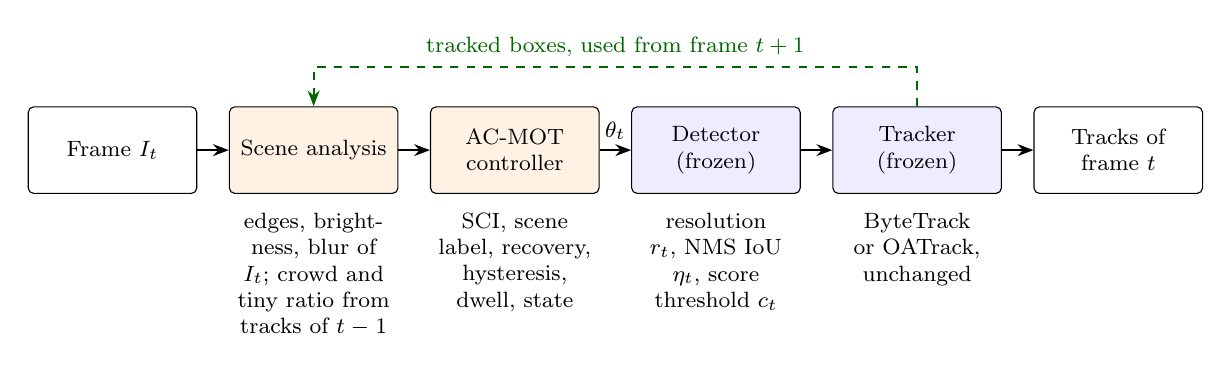
\begin{tikzpicture}[
  font=\footnotesize,
  node distance=4mm,
  stage/.style={draw, rounded corners=2pt, align=center, text width=20mm,
                minimum height=11mm, inner sep=2pt},
  ctrl/.style={stage, fill=orange!10},
  host/.style={stage, fill=blue!7},
  note/.style={align=center, text width=22.5mm, font=\footnotesize, inner sep=1pt},
  arr/.style={-{Stealth[length=2mm]}, thick},
  fb/.style={-{Stealth[length=2mm]}, thick, dashed, green!40!black}]
\node[stage] (frame) {Frame $I_t$};
\node[ctrl, right=of frame] (scene) {Scene analysis};
\node[ctrl, right=of scene] (ctrl) {AC-MOT\\controller};
\node[host, right=of ctrl] (det) {Detector\\(frozen)};
\node[host, right=of det] (trk) {Tracker\\(frozen)};
\node[stage, right=of trk] (out) {Tracks of\\frame $t$};
\draw[arr] (frame) -- (scene);
\draw[arr] (scene) -- (ctrl);
\draw[arr] (ctrl) -- node[above, font=\footnotesize] {$\theta_t$} (det);
\draw[arr] (det) -- (trk);
\draw[arr] (trk) -- (out);
\node[note, below=2mm of scene] {edges, brightness, blur of $I_t$; crowd and tiny ratio from tracks of $t-1$};
\node[note, below=2mm of ctrl] {SCI, scene label, recovery, hysteresis, dwell, state};
\node[note, below=2mm of det] {resolution $r_t$, NMS IoU $\eta_t$, score threshold $c_t$};
\node[note, below=2mm of trk] {ByteTrack or OATrack, unchanged};
\draw[fb] (trk.north) -- ++(0,5mm) -| node[pos=0.25, above, font=\footnotesize]
  {tracked boxes, used from frame $t+1$} (scene.north);
\end{tikzpicture}
\caption{AC-MOT in a tracking-by-detection pipeline. Scene analysis and the
controller choose the operating point $\theta_t=(c_t,\eta_t,r_t)$ before the
detector runs. The frozen detector and tracker are not modified. Tracked boxes
of frame $t$ feed the scene analysis of later frames (dashed arrow).}
\label{fig:pipeline}
\end{figure*}

\begin{table}[t]
\caption{Symbols computed at run time. Fixed values are listed in
Table~\ref{tab:constants}.}
\label{tab:symbols}
\centering\footnotesize
\setlength{\tabcolsep}{4pt}
\begin{tabular}{@{}l>{\raggedright\arraybackslash}p{55mm}@{}}
\toprule
Symbol & Meaning\\
\midrule
$t$ & frame index\\
$j$ & analysis step (frames $1, 11, 21, \dots$)\\
$I_t$ & image of frame $t$\\
$r_t$, $\eta_t$, $c_t$ & input resolution, NMS IoU threshold, score threshold
  used at frame $t$, Eq.~\eqref{eq:theta}\\
$\mathcal{B}_{1:t-1}$ & boxes reported by the tracker for frames $1$ to $t-1$\\
$e_t$, $\beta_t$, $\nu_t$ & edge density, brightness, and sharpness of $I_t$\\
$N_j$ & number of tracked boxes in frame $t-1$\\
$a_i$ & area of tracked box $i$ in pixels\\
$C_j$ & crowd cue, Eq.~\eqref{eq:crowd}\\
$T_j$ & tiny-object ratio, Eq.~\eqref{eq:tiny}\\
$S_j$ & scene complexity index (SCI), Eq.~\eqref{eq:sci}\\
$H_j$ & the last seven analysis steps\\
$\ell_j$ & scene label, Eq.~\eqref{eq:label}\\
$g_j$ & target state, Eqs.~\eqref{eq:target}--\eqref{eq:hold}\\
$q_j$ & controller state: LOW, MEDIUM, or HIGH, Eq.~\eqref{eq:dwell}\\
$P_j$, $d_j$ & peak object count and drop counter,
  Eqs.~\eqref{eq:drop}--\eqref{eq:peak}\\
$t_c$ & frame of the last state change\\
\bottomrule
\end{tabular}
\end{table}

\subsection{Scene cues}
Scene analysis does not run on every frame. It runs on frame 1 and then once
every 10 frames ($t=1$ or $t \bmod 10 = 1$, that is, frames 1, 11, 21,
\dots). Each of these frames is an analysis step $j$. Between two analysis
steps the controller keeps its last decision. The stride of 10 frames was
selected by a temporal sweep on validation data (Sect.~\ref{sec:constants}).
Two kinds of cues are computed at each step.

\emph{Image cues of the current frame.} The frame is reduced to a quarter of
its width and height and converted to gray levels, so that the cues are cheap
to compute. Three cues are then measured:
\begin{itemize}
\item the edge density $e_t$, the fraction of pixels marked as edges by the
      Canny detector (lower and upper thresholds 50 and 120); many edges
      indicate a cluttered scene;
\item the brightness $\beta_t$, the mean gray level from 0 (black) to 255
      (white); a low value indicates a dark or night scene;
\item the sharpness $\nu_t$, the variance of the Laplacian of the gray image;
      a low value indicates a blurred frame.
\end{itemize}

\emph{Box cues of the previous frame.} Let $N_j$ be the number of boxes that
the tracker reported for frame $t-1$, and let $a_i$ be the area of box $i$ in
pixels of the original image. The crowd cue and the tiny-object ratio are
\begin{align}
C_j&=\min\!\left(\frac{N_j}{30},1\right),\label{eq:crowd}\\
T_j&=\frac{1}{N_j}\sum_{i=1}^{N_j}\mathbf{1}\!\left[a_i<32^2\right].\label{eq:tiny}
\end{align}
$C_j$ is the number of tracked objects divided by 30 and capped at 1, so every
frame with 30 or more objects has $C_j=1$. $T_j$ is the fraction of tracked
boxes smaller than $32\times32$ pixels, which is the size limit of small
objects in the COCO benchmark \cite{lin2014coco}. The indicator
$\mathbf{1}[\cdot]$ is 1 when its condition holds and 0 otherwise, and $T_j=0$
when $N_j=0$.

\subsection{Scene complexity index and scene label}
The scene complexity index (SCI) measures how crowded the recent frames are.
It is the mean crowd cue of the last seven analysis steps:
\begin{equation}
S_j=\frac{1}{|H_j|}\sum_{k\in H_j} C_k,
\label{eq:sci}
\end{equation}
where $H_j$ holds the steps $j-6,\dots,j$ (fewer at the start of a video) and
$|H_j|$ is their number. With a stride of 10 frames, the seven steps cover
about the last 60 frames, so a single unusual frame changes $S_j$ only a little. The
window of seven steps was selected by the same temporal sweep as the stride
(Sect.~\ref{sec:constants}). Because $C_j\le1$, $S_j$ lies between 0 and 1.
While fewer than 30 objects are tracked, $S_j$ is simply the recent average
number of tracked objects divided by 30.

The SCI uses the crowd cue alone. During development, all 31 combinations of
the five cues (crowd, tiny ratio, edges, brightness, and blur) were tested as
SCI inputs on the calibration sequences, and the crowd cue alone was selected
(Sect.~\ref{sec:modern}). The other four cues are still used as checks on the
state through the scene label
\begin{equation}
\ell_j=\begin{cases}
\text{night}   & \text{if } \beta_t<80,\\
\text{blur}    & \text{else if } \nu_t<180,\\
\text{tiny}    & \text{else if } T_j>0.50,\\
\text{crowded} & \text{else if } C_j>0.65 \text{ or } e_t>0.13,\\
\text{clear}   & \text{otherwise.}
\end{cases}
\label{eq:label}
\end{equation}
The conditions are checked from top to bottom, and the first one that holds
gives the label. For example, $T_j>0.50$ means that more than half of the
tracked boxes are tiny, and $C_j>0.65$ means that at least 20 objects are
tracked.

\subsection{Three-state controller}
The controller is always in one of three states: LOW, MEDIUM, or HIGH. The
names describe how difficult the scene is. They do not rank the input size:
in the final action map the HIGH state uses the smallest input
(Table~\ref{tab:actions}). The state changes only at analysis steps, in four
steps (Algorithm~\ref{alg:controller}).

\emph{Step 1: target state.} The SCI and the scene label give a target state
\begin{equation}
g_j=\begin{cases}
\text{HIGH}   & \text{if } S_j>\tau_h \text{ or } T_j>0.50,\\
\text{MEDIUM} & \text{else if } S_j>\tau_m \text{ or}\\
              & \quad \ell_j\in\{\text{crowded},\text{tiny}\},\\
\text{LOW}    & \text{otherwise,}
\end{cases}
\label{eq:target}
\end{equation}
where $\tau_m=0.297$ and $\tau_h=0.511$ are the two SCI thresholds (exact
values in Table~\ref{tab:constants}). They were selected by the joint search
on the calibration sequences (Sect.~\ref{sec:constants}). Since $S_j$ is the
recent average number of tracked objects divided by 30, the SCI conditions
give MEDIUM above about 9 objects ($30\tau_m=8.9$) and HIGH above about 15
objects ($30\tau_h=15.3$).

\emph{Step 2: recovery probe.} When the number of tracked objects suddenly
collapses, the controller tries the HIGH action for a short time. It keeps a
slowly decaying peak $P_j$ of the object count and a drop counter $d_j$:
\begin{align}
d_j&=\begin{cases}
d_{j-1}+1 & \text{if } P_{j-1}\ge5 \text{ and}\\
          & \quad N_j<0.40\,P_{j-1},\\
0         & \text{otherwise,}
\end{cases}\label{eq:drop}\\
P_j&=\max\left(N_j,\lfloor 0.8\,P_{j-1}\rfloor\right),\label{eq:peak}
\end{align}
with $P_0=d_0=0$. A collapse is detected when at least 5 objects were seen
before and fewer than 40\% of them remain. The peak loses 20\% at each step,
so an old peak is forgotten after a few steps. While $1\le d_j\le3$, the
target $g_j$ is set to HIGH, so the probe lasts at most three analysis steps
(30 frames).

\emph{Step 3: hysteresis.} A move to a lower state is held while the scene is
still close to difficult:
\begin{equation}
g_j\leftarrow\begin{cases}
\text{HIGH}   & \text{if } q_{j-1}=\text{HIGH} \text{ and}\\
              & \quad (S_j>0.50 \text{ or } T_j>0.40),\\
\text{MEDIUM} & \text{if } q_{j-1}=\text{MEDIUM},\\
              & \quad g_j=\text{LOW} \text{ and } S_j>0.25,\\
g_j           & \text{otherwise.}
\end{cases}
\label{eq:hold}
\end{equation}
The hold values lie just below the values that lead into each state
($0.50<\tau_h$, 0.40 below the tiny guard of 0.50, and $0.25<\tau_m$),
so the state does not jump back and forth when the scene stays near a
threshold. Upward moves are not held.

\emph{Step 4: dwell.} After a change, the state is kept for at least 30 frames,
that is, three analysis steps:
\begin{equation}
q_j=\begin{cases}
g_j     & \text{if } t-t_c\ge30,\\
q_{j-1} & \text{otherwise,}
\end{cases}
\label{eq:dwell}
\end{equation}
where $t_c$ is the frame of the last state change. The controller starts in
LOW with $t_c=1$, so the first change is possible at frame 31. Whenever
$q_j\ne q_{j-1}$, $t_c$ is set to $t$.

The state $q_j$ then selects the operating point from the action map, and the
detector uses it until the next analysis step.

\begin{algorithm}[t]
\caption{AC-MOT controller for one video}\label{alg:controller}
\begin{algorithmic}[1]
\State $q\gets$ LOW; $H\gets\emptyset$; $P\gets0$; $d\gets0$; $t_c\gets1$
\For{each frame $t=1,2,\dots$}
  \If{$t=1$ \textbf{or} $t \bmod 10=1$}
    \State $e_t,\beta_t,\nu_t\gets$ image cues of $I_t$
    \State $N,C,T\gets$ box cues of frame $t-1$
    \State add $C$ to $H$ (keep 7); $S\gets\mathrm{mean}(H)$
    \State $\ell\gets$ label (Eq.~\ref{eq:label}); $g\gets$ target (Eq.~\ref{eq:target})
    \State update $d$ and $P$ (Eqs.~\ref{eq:drop}--\ref{eq:peak})
    \If{$1\leq d\leq3$} $g\gets$ HIGH
    \EndIf
    \State apply the holds (Eq.~\ref{eq:hold})
    \If{$t-t_c\geq30$ \textbf{and} $g\neq q$}
      \State $q\gets g$; $t_c\gets t$
    \EndIf
  \EndIf
  \State $(r_t,\eta_t,c_t)\gets$ action of state $q$ (Table~\ref{tab:actions})
  \State detect with $(r_t,\eta_t)$; drop scores $<c_t$
  \State update the tracker; store its boxes
\EndFor
\end{algorithmic}
\end{algorithm}

\subsection{Action map}
Table~\ref{tab:actions} gives the operating point of each state. LOW uses the
largest input (1536 pixels), loose NMS (0.70), and a low score threshold
(0.10), so the detector passes more weak boxes when the scene is sparse.
MEDIUM uses 1280 pixels, tight NMS (0.45), and a score threshold of 0.40.
HIGH uses 1088 pixels, NMS 0.60, and a score threshold of 0.40. In the two
difficult states, the detector therefore passes only boxes with a score of at
least 0.40. The map was selected together with $\tau_m$ and $\tau_h$ by the
joint search on the calibration sequences (Sect.~\ref{sec:constants}). The
score threshold $c_t$ is applied on the detector side before the tracker. It is
separate from any confidence gate inside the tracker, such as the fixed
tracker-side gate of OATrack.

\begin{table}[t]
\caption{Action map. State names describe scene difficulty, not a resolution
rank. Selected by the joint search on the calibration sequences.}
\label{tab:actions}
\centering\footnotesize
\begin{tabular}{@{}lrrr@{}}
\toprule
State & Resolution $r$ & NMS IoU $\eta$ & Score threshold $c$\\
\midrule
LOW & 1536 & 0.70 & 0.10\\
MEDIUM & 1280 & 0.45 & 0.40\\
HIGH & 1088 & 0.60 & 0.40\\
\bottomrule
\end{tabular}
\end{table}

\subsection{How each value was chosen}\label{sec:constants}
All values of Tables~\ref{tab:actions} and~\ref{tab:constants} were fixed
before the final evaluation and were not changed after it. The last column of
Table~\ref{tab:constants} gives the source of each value. There are four
sources.

\emph{Joint search on the calibration sequences.} The SCI thresholds $\tau_m$
and $\tau_h$ and the action map were selected together by an Optuna TPE search
with 60 trials \cite{akiba2019optuna}. The calibration sequences are eight
sequences of the VisDrone2019-MOT training split. They serve as the validation
(tuning) data of the final stage and are disjoint from the evaluation
sequences. Each trial was scored by four-fold cross-validation, with two
sequences held out in each fold, as the mean change in HOTA against the
baseline. The search ranges were $\tau_m\in[0.10,0.50]$ and
$\tau_h\in[\tau_m+0.05,\min(\tau_m+0.40,0.90)]$, with, for each state, an
input of 1088, 1280, or 1536 pixels, an NMS value of 0.45, 0.60, or 0.70,
and a score threshold of 0.10, 0.25, or 0.40. The input sizes and NMS values
are the operating points for which detector outputs were cached; 1536 pixels
with NMS 0.70 is the baseline point, and 0.70 is the default NMS value of the
Ultralytics detector. The three score thresholds are the low and high
thresholds of ByteTrack (0.10 and 0.25) and the confidence gate of OATrack
(0.40). In a separate sweep of the score threshold over 0.01, 0.10, 0.25, and
0.40 on the same sequences, at 1088 pixels and NMS 0.45, 0.40 gave the highest
pooled HOTA (+0.881 over 0.01) and improved seven of the eight sequences. The frozen policy reached a mean HOTA
gain of 2.447 points over the four folds, with all folds positive
(Sect.~\ref{sec:modern}).

\emph{Cue audit on the calibration sequences.} The choice of the crowd cue as
the only SCI input came from testing all 31 non-empty subsets of the five
cues with the same cross-validation (Sect.~\ref{sec:modern}).

\emph{Temporal sweep on the validation split.} The analysis stride and the
SCI window were selected in the first development stage, with the YOLOv8n
pipeline, on the VisDrone2019-MOT validation sequences. The sweep tested 25
combinations: windows of 1, 3, 5, 7, and 9 analysis steps and strides of 1, 5,
10, 15, and 20 frames. Five of the 25 settings met both constraints of that
stage, at least 25 FPS and at most 271 IDS (the IDS of the original controller
on the same data). Among them, a window of 7 and a stride of 10 gave the
highest MOTA, 18.165 against 18.044 for the next setting. Operating-point
sweeps on the same data covered input resolutions from 512 to 960 pixels,
confidence thresholds from 0.05 to 0.50, and NMS thresholds from 0.30 to 0.80,
and defined the supported values of the first optimized profiles
(Sect.~\ref{sec:development}).

\emph{Fixed design values.} The tiny-object area follows the COCO definition
of small objects \cite{lin2014coco}. The remaining values (the crowd
normalizer, the Canny thresholds, the label thresholds, the recovery, hold,
and dwell values, and the initial state) come from the original AC-MOT
controller and were kept unchanged in every search of the final stage. The
searched values above
were tuned with these values in place, so the selected thresholds and actions
are matched to them. For example, the crowd normalizer of 30 only sets the
scale of $S_j$: $\tau_m$ and $\tau_h$ were searched on this scale and
correspond to about 9 and 15 tracked objects.

\begin{table*}[t]
\caption{Values of the AC-MOT controller and how each value was chosen.
Calibration sequences: eight VisDrone2019-MOT training sequences used as
tuning data, disjoint from the evaluation sequences. CV: four-fold
cross-validation.}
\label{tab:constants}
\centering\footnotesize
\setlength{\tabcolsep}{4pt}
\begin{tabular}{@{}l>{\raggedright\arraybackslash}p{50mm}l>{\raggedright\arraybackslash}p{62mm}@{}}
\toprule
Symbol & Meaning & Value & How the value was chosen\\
\midrule
$\tau_m$ & SCI threshold for MEDIUM, Eq.~\eqref{eq:target} & 0.29747709701135766 & joint TPE search on the calibration sequences, 60 trials, CV\\
$\tau_h$ & SCI threshold for HIGH, Eq.~\eqref{eq:target} & 0.5114928923560124 & same joint search\\
$(r,\eta,c)$ & operating point of each state & Table~\ref{tab:actions} & same joint search over $\{1088,1280,1536\}\times\{0.45,0.60,0.70\}\times\{0.10,0.25,0.40\}$\\
-- & SCI input cue & crowd only & cue audit of all 31 cue subsets on the calibration sequences, CV\\
-- & analysis stride & 10 frames & temporal sweep of 25 settings on the validation split; highest MOTA with $\geq$25 FPS and $\leq$271 IDS\\
$|H_j|$ & SCI window & 7 steps & same temporal sweep\\
-- & tiny-object area & $32\times32$ pixels & COCO small-object limit \cite{lin2014coco}\\
-- & crowd normalizer, Eq.~\eqref{eq:crowd} & 30 boxes & original controller; sets the scale on which $\tau_m$, $\tau_h$ were searched\\
-- & Canny thresholds (lower, upper) & 50, 120 & original controller; fixed in all final-stage searches\\
-- & night and blur labels, Eq.~\eqref{eq:label} & $\beta_t<80$, $\nu_t<180$ & original controller; fixed in all final-stage searches\\
-- & crowded label, Eq.~\eqref{eq:label} & $C_j>0.65$ or $e_t>0.13$ & original controller; fixed in all final-stage searches\\
-- & tiny label and HIGH guard, Eqs.~\eqref{eq:label}, \eqref{eq:target} & $T_j>0.50$ & original controller; fixed in all final-stage searches\\
-- & recovery: minimum peak, drop ratio, peak decay, steps & 5, 0.40, 0.80, 3 & original controller; fixed in all final-stage searches\\
-- & holds in HIGH ($S_j$, $T_j$) and MEDIUM ($S_j$), Eq.~\eqref{eq:hold} & (0.50, 0.40), 0.25 & original controller; fixed in all final-stage searches\\
-- & dwell, Eq.~\eqref{eq:dwell} & 30 frames & original controller; fixed in all final-stage searches\\
-- & initial state & LOW & original controller; fixed in all final-stage searches\\
\bottomrule
\end{tabular}
\end{table*}
\section{How the Final Controller Was Developed}\label{sec:development}

The controller was developed in four steps: a quality-oriented profile, an
identity-aware profile, transfer and cross-pipeline studies, and a modern
stage that produced the frozen controller. Each step is compared with the
baseline it was built on. The historical steps used other detectors and
evaluation protocols than the modern stage, so their numbers are reported in
their own tables and are not pooled with the modern results.

\subsection{Quality-oriented profile}\label{sec:quality}

\emph{Baseline.} The reference pipeline is the pretrained YOLOv8n detector
\cite{jocher2023yolov8} followed by ByteTrack \cite{zhang2022bytetrack}, both at
their default settings: confidence threshold 0.25, NMS IoU threshold 0.45,
input size 640 pixels, and the default ByteTrack parameters (high threshold
0.25, low threshold 0.10, new-track threshold 0.25, buffer 30 frames, match
threshold 0.80). It runs with one fixed operating point for the whole video.

\emph{Method.} The first optimization-derived profile kept the same detector,
used a tuned ByteTrack profile, and searched only on the VisDrone2019-MOT
validation split. Five cues were used: crowd count, the fraction of earlier
boxes below $32\times32$ pixels, edge density, low brightness, and low
Laplacian variance. Each cue was normalized with validation statistics, and
the index was their weighted sum
\begin{equation}
S_j=\sum_{k\in\{c,t,e,n,b\}}w_k\,x_{k,j},
\label{eq:hist-sci}
\end{equation}
where $k$ runs over the five cues (c: crowd, t: tiny ratio, e: edges, n: low
brightness, b: blur), $x_{k,j}$ is the normalized value of cue $k$ at analysis
step $j$, and $w_k$ is its weight, with $w_k\geq0$ and $\sum_k w_k=1$. The
index was averaged over seven analyses taken every ten frames. Confidence and NMS were interpolated linearly between the values
at $S=0$ and $S=1$, and two sorted thresholds selected one of three
resolutions (512, 928, 960 pixels).

An Optuna TPE study \cite{akiba2019optuna} jointly searched the five weights,
the confidence and NMS end points, and the two thresholds. The resolution
levels, the supported confidence values $\{0.25,\dots,0.45\}$, the supported
NMS values from 0.30 to 0.70, and the temporal settings were fixed beforehand
by validation sweeps (Sect.~\ref{sec:constants}). The selection rule kept
trials with at least 25 FPS and at most 271 IDS (the IDS of the original
controller on the same validation data) and then took the highest MOTA, with lower IDS, HOTA,
IDF1, and FPS as tie-breaks. The frozen profile (archived as Trial~24) has
$w_c=0.1294928$, $w_t=0.2217477$, $w_e=0.4337134$, $w_n=0.0535577$,
$w_b=0.1614885$, confidence end points $(0.30,0.40)$, NMS end points
$(0.35,0.35)$, and thresholds $(0.1353494, 0.2872868)$. On validation it
reached MOTA 23.038, HOTA 36.110, IDF1 40.758, and IDS 270 at 37.169 FPS.

\emph{Comparison.} Table~\ref{tab:quality} compares the profile with the
baseline on the historical VisDrone test-dev split, with paired bootstrap
intervals (5000 resamples, seed 42). HOTA rises by 5.4051 points, MOTA by
7.2195 points, and IDF1 by 8.8220 points, and throughput rises from 36.528 to
38.985 FPS.

\begin{table}[t]
\caption{Quality-oriented profile versus its baseline (YOLOv8n with ByteTrack
at default settings) on VisDrone test-dev, historical protocol. Gain: paired
bootstrap difference with 95\% interval; for IDS it is the reduction.}
\label{tab:quality}
\centering\footnotesize
\setlength{\tabcolsep}{4pt}
\begin{tabular}{@{}lrrl@{}}
\toprule
Metric & Baseline & Quality & Gain [95\% CI]\\
\midrule
HOTA & 28.430 & 33.835 & $+5.4051$ $[4.1273, 6.9022]$\\
MOTA & 19.729 & 26.948 & $+7.2195$ $[5.4362, 9.2934]$\\
IDF1 & 32.724 & 41.546 & $+8.8220$ $[6.9005, 11.0537]$\\
IDS & 1235 & 1184 & $51$ $[-114, 219]$\\
FPS & 36.528 & 38.985 & --\\
\bottomrule
\end{tabular}
\end{table}

\subsection{Identity-aware Pareto profile}\label{sec:identity}

\emph{Baseline.} The baseline is the same YOLOv8n and ByteTrack pipeline at
default settings (Sect.~\ref{sec:quality}).

\emph{Method.} Quality is not the only deployment goal; identity stability and
compute can move in a different direction from MOTA. The second study kept
the same cues, operating levels, temporal settings, and validation data, but
changed the question. It maximized MOTA and minimized IDS subject only to
$\mathrm{FPS}\geq25$, without the IDS gate. A seeded TPE sampler ran 49
completed trials. A trial dominated another when it had no lower MOTA and no
higher IDS, with at least one strict improvement, and the feasible Pareto
front was built from these relations. The balanced
candidate maximized an equal-weight score of normalized MOTA and normalized IDS
reduction, with HOTA, IDF1, FPS, and trial index as tie-breaks.

The selected profile (archived as Trial~22) has weights $w_c=0.1646453$,
$w_t=0.1746265$, $w_e=0.5076113$, $w_n=0.1206956$, $w_b=0.0324213$,
confidence end points $(0.40,0.40)$, NMS end points $(0.60,0.35)$, and
thresholds $(0.2927136, 0.6661672)$. On validation it reached MOTA 19.330,
HOTA 31.651, IDF1 34.226, and IDS 168 at 51.406 FPS.

\emph{Comparison.} Table~\ref{tab:identity} compares the profile with the
baseline on test-dev. It removes 316 identity switches and raises throughput
from 36.528 to 46.024 FPS, while HOTA, MOTA, and IDF1 also rise. Against the
quality-oriented profile it has 265 fewer IDS $[82, 502]$ and $-2.617$ HOTA
$[-4.004, -1.694]$. The two profiles therefore answer different questions: one
favors overall quality and the other favors identity stability and speed.

\begin{table}[t]
\caption{Identity-aware profile versus its baseline (YOLOv8n with ByteTrack at
default settings) on VisDrone test-dev, historical protocol. Gain: paired
bootstrap difference with 95\% interval; for IDS it is the reduction.}
\label{tab:identity}
\centering\footnotesize
\setlength{\tabcolsep}{4pt}
\begin{tabular}{@{}lrrl@{}}
\toprule
Metric & Baseline & Identity & Gain [95\% CI]\\
\midrule
HOTA & 28.430 & 31.218 & $+2.788$ $[0.747, 4.660]$\\
MOTA & 19.729 & 23.792 & $+4.063$ $[0.952, 6.886]$\\
IDF1 & 32.724 & 37.870 & $+5.146$ $[2.028, 8.080]$\\
IDS & 1235 & 919 & $316$ $[175, 470]$\\
FPS & 36.528 & 46.024 & --\\
\bottomrule
\end{tabular}
\end{table}

\subsection{Transfer and cross-pipeline studies}\label{sec:transfer}

\emph{UAVDT.} The baseline is again YOLOv8n with ByteTrack at default settings
(Sect.~\ref{sec:quality}). Both frozen profiles were applied to UAVDT
\cite{du2018uavdt} without retuning (Table~\ref{tab:hist-uavdt}). The
quality-oriented profile raised HOTA by 4.305 points $[2.740, 5.709]$ and the
identity-aware profile by 2.845 points $[1.238, 4.348]$; their IDS reductions
are 237 $[104, 377]$ and 250 $[110, 404]$.

\begin{table}[t]
\caption{Historical UAVDT transfer without retuning. Baseline: YOLOv8n with
ByteTrack at default settings.}
\label{tab:hist-uavdt}
\centering\footnotesize
\setlength{\tabcolsep}{4pt}
\begin{tabular}{@{}lrrr@{}}
\toprule
Metric & Baseline & Quality & Identity\\
\midrule
HOTA & 24.085 & 28.390 & 26.930\\
MOTA & 13.841 & 17.399 & 16.118\\
IDF1 & 27.887 & 34.453 & 32.014\\
IDS & 558 & 321 & 308\\
FPS & 65.015 & 58.353 & 61.462\\
\bottomrule
\end{tabular}
\end{table}

\emph{U2MOT on VisDrone.} The baseline is the published U2MOT tracker
\cite{liu2023u2mot} with its released YOLOX-X detector, run
at its own static setting. Seven VisDrone validation sequences served for
development and 17 test-dev sequences for evaluation. The cue weights and
transforms of the quality-oriented profile were kept, the tracker was not
modified, and the action boundaries were set to the 33rd and 67th percentiles
of the index on the U2MOT validation run, without using ground truth.
Table~\ref{tab:u2mot} gives the comparison: the controlled pipeline has 87
fewer IDS and 1230 fewer FP.

\begin{table}[t]
\caption{Cross-pipeline study on VisDrone test-dev. Baseline: U2MOT with its
YOLOX-X detector at its static setting.}
\label{tab:u2mot}
\centering\footnotesize
\setlength{\tabcolsep}{4pt}
\begin{tabular}{@{}lrr@{}}
\toprule
Metric & U2MOT baseline & With controller\\
\midrule
MOTA & 53.873 & 53.767\\
IDF1 & 69.775 & 69.849\\
IDS & 1239 & 1152\\
FP & 41385 & 40155\\
FN & 63241 & 64801\\
\bottomrule
\end{tabular}
\end{table}

\emph{SparseTrack on MOT17.} The baseline is the published SparseTrack tracker
\cite{liu2025sparsetrack} with a fixed NMS IoU threshold of 0.75, on the seven
MOT17 \texttt{val\_half} sequences (2652 frames) \cite{dendorfer2021motchallenge}.
A minimal edge-driven rule switched only the NMS threshold, between 0.70 and
0.80; its threshold came from a leave-one-sequence-out study on the same
sequences. Table~\ref{tab:sparsetrack} gives the comparison: the adaptive rule
reduces IDS from 136 to 123, with MOTA $+0.0371$ points $[-0.041, +0.182]$.

\begin{table}[t]
\caption{Cross-pipeline study on MOT17 \texttt{val\_half}. Baseline:
SparseTrack with a fixed NMS IoU threshold of 0.75.}
\label{tab:sparsetrack}
\centering\footnotesize
\setlength{\tabcolsep}{4pt}
\begin{tabular}{@{}lrr@{}}
\toprule
Metric & SparseTrack baseline & With adaptive NMS\\
\midrule
MOTA & 76.8881 & 76.9252\\
IDF1 & 81.4943 & 81.5299\\
IDS & 136 & 123\\
\bottomrule
\end{tabular}
\end{table}

Together these studies show that the preferred profile depends on the
objective (quality or identity) and on the tracker host. This motivated a
modern stage with a stronger detector, explicit calibration data, and two
tracker hosts.

\subsection{Modern development of the frozen controller}\label{sec:modern}

\emph{Baseline.} The modern baseline is the YOLO11m detector
\cite{jocher2024yolo11}, in the public VisDrone checkpoint described in
Sect.~\ref{sec:hosts}, run at a fixed operating point of 1536 pixels and NMS
IoU 0.70 with no extra score threshold. It feeds ByteTrack
\cite{zhang2022bytetrack} during development and both ByteTrack and OATrack
\cite{qi2026oatrack} in the final evaluation. A large fixed input is a common
choice for small aerial objects when no adaptation is used.

\emph{Data and protocol.} Eight sequences of the VisDrone2019-MOT training split
(3282 frames) were declared as calibration data. They are disjoint from the
seven evaluation sequences. All development used four folds, each holding out
two calibration sequences, and reported the cross-validated (CV) mean change
in HOTA against the baseline. Detector outputs were cached for every
resolution and NMS value; a score threshold applied to the cache was checked
to reproduce direct inference exactly. Table~\ref{tab:devrecord} summarizes
the development steps.

\emph{Cue audit.} Stages 1 and 2 searched the state-to-resolution and
state-to-NMS maps on exhaustive grids. Stage 3A searched all 31 non-empty
subsets of the five cues and selected \{crowd\}, which defines the
crowd-selected SCI of Eq.~\eqref{eq:sci}. The other cues were kept as guard and
auxiliary cues of the state logic (Sect.~\ref{sec:method}).

\emph{Score threshold.} At 1088 pixels and NMS 0.45, a fixed score threshold
of 0.40 raised pooled calibration HOTA by $+0.881$ over 0.01 and improved
seven of the eight sequences. The score threshold was therefore added as the
third action dimension.

\emph{Final joint search.} The final search used 60 TPE trials (seed 43). It
searched $\tau_m\in[0.10,0.50]$, $\tau_h\in[\tau_m+0.05,\min(\tau_m+0.40,0.90)]$,
and for each state a resolution in $\{1088,1280,1536\}$, an NMS value in
$\{0.45,0.60,0.70\}$, and a score threshold in $\{0.10,0.25,0.40\}$. The
objective was the CV mean change in HOTA against the baseline, with ByteTrack
as host. Eligible candidates had to realize at least two distinct actions,
each on at least 10\% of calibration frames, and switch within sequences. The
frozen policy is the eligible candidate whose three states use three
different actions (Table~\ref{tab:actions}). On calibration data it used LOW,
MEDIUM, and HIGH on 7.6\%, 10.1\%, and 82.3\% of frames, with 0.607 state
changes per 100 frames on average.

\emph{Comparison.} Table~\ref{tab:folds} compares the frozen policy with the
baseline on each calibration fold. All four folds are positive, with a CV
mean of $+2.447$ HOTA. After these steps the thresholds, cue subset, and
action map were frozen. The final comparison on the evaluation sequences is
given in Sect.~\ref{sec:results}.

\begin{table}[t]
\caption{Main modern development steps on the eight calibration sequences
(ByteTrack host). The score-threshold gain is pooled HOTA; the joint-search
result is the mean over four folds.}
\label{tab:devrecord}
\centering\footnotesize
\setlength{\tabcolsep}{3pt}
\begin{tabular}{@{}lll@{}}
\toprule
Step & Search & Result\\
\midrule
Cue subset & 31 subsets & \{crowd\}\\
Score threshold & 4 values & 0.40; $+0.881$ HOTA\\
Joint search & 60 TPE trials & CV mean $+2.447$\\
\bottomrule
\end{tabular}
\end{table}

\begin{table}[t]
\caption{Frozen policy versus the modern baseline (YOLO11m at 1536 pixels and
NMS 0.70, ByteTrack) on the four calibration folds: change in HOTA.}
\label{tab:folds}
\centering\footnotesize
\begin{tabular}{@{}lrrrrr@{}}
\toprule
 & Fold 1 & Fold 2 & Fold 3 & Fold 4 & Mean\\
\midrule
$\Delta$HOTA & $+0.592$ & $+4.164$ & $+2.029$ & $+3.004$ & $+2.447$\\
\bottomrule
\end{tabular}
\end{table}
\section{Results}\label{sec:results}

All experiments use the YOLO11m detector of Sect.~\ref{sec:hosts}. It runs in
half precision, and detections of the classes pedestrian, car, van, truck, and
bus are passed on. ByteTrack uses the Ultralytics implementation with its
default parameters: high threshold 0.25, low threshold 0.10, new-track
threshold 0.25, buffer 30 frames, and match threshold 0.80. OATrack is a
re-implementation of the published method \cite{qi2026oatrack} in its main
configuration, with its published tracker-side confidence gate of 0.40. This
gate belongs to the tracker and is never changed by AC-MOT. For each host, two
systems are compared. The baseline runs the detector at the fixed operating
point of 1536 pixels and NMS IoU 0.70, with a minimal score threshold of 0.01.
This is the largest input of the operating-point grid, and 0.70 is the default
NMS value of the Ultralytics detector. AC-MOT runs the frozen controller of
Sect.~\ref{sec:method} on the same detector. The two systems differ only in
the detector operating point. Uncertainty is estimated with the paired
bootstrap of Sect.~\ref{sec:metrics}, with 5000 resamples (seed 42).
Latency is measured on one Tesla T4 GPU over the first 200 frames of sequence
\texttt{uav0000086\_00000\_v}, excluding five warm-up frames. For every
frame, the time spent in the controller (image statistics, scene analysis, and
state update) is recorded separately from the detector and tracker time.

\subsection{Frozen VisDrone evaluation}
The VisDrone evaluation uses seven sequences of the VisDrone2019-MOT
validation split. They contain 71,830 ground-truth boxes. The cue subset,
thresholds, and action map of the frozen controller were selected on the
separate calibration sequences only (Sect.~\ref{sec:modern}). Results are
scored with a Python port of the VisDrone2019-MOT Task~4b evaluation. Ignored
regions are removed, the five classes above are evaluated separately,
CLEAR-MOT and identity measures use IoU 0.5, and counts are summed over
classes and sequences. HOTA is added with the same class-aware scheme using
TrackEval. The bootstrap draws seven sequences with replacement.

Table~\ref{tab:visdrone} lists the aggregate results on the seven VisDrone
sequences, and Fig.~\ref{fig:visdrone} shows HOTA, MOTA, and IDF1.

\begin{table}[t]
\caption{Frozen VisDrone evaluation on seven VisDrone2019-MOT sequences
(71,830 ground-truth boxes). Baseline: fixed operating point (1536, 0.70).}
\label{tab:visdrone}
\centering\footnotesize
\setlength{\tabcolsep}{4pt}
\begin{tabular}{@{}lrrrr@{}}
\toprule
 & \multicolumn{2}{c}{ByteTrack} & \multicolumn{2}{c}{OATrack}\\
\cmidrule(lr){2-3}\cmidrule(l){4-5}
Metric & Baseline & AC-MOT & Baseline & AC-MOT\\
\midrule
HOTA & 41.586 & 44.523 & 46.770 & 48.095\\
MOTA & 9.876 & 27.871 & 28.165 & 34.483\\
IDF1 & 48.569 & 53.929 & 57.107 & 59.364\\
IDS & 1341 & 1016 & 773 & 604\\
FP & 39274 & 24892 & 25394 & 21400\\
FN & 24121 & 25902 & 25432 & 25057\\
Precision & 54.849 & 64.852 & 64.628 & 68.609\\
Recall & 66.419 & 63.940 & 64.594 & 65.116\\
\bottomrule
\end{tabular}
\end{table}

\emph{ByteTrack host.} AC-MOT changes HOTA from 41.586 to 44.523, MOTA from
9.876 to 27.871, and IDF1 from 48.569 to 53.929. IDS fall from 1341 to 1016
and FP from 39274 to 24892, while FN rise from 24121 to 25902. Precision rises
from 54.849 to 64.852 and recall falls from 66.419 to 63.940. The detector
output becomes more selective: clutter and identity-confusing boxes are
removed at a small cost in recall.

\emph{OATrack host.} AC-MOT changes HOTA from 46.770 to 48.095, MOTA from
28.165 to 34.483, and IDF1 from 57.107 to 59.364. IDS fall from 773 to 604, FP
from 25394 to 21400, and FN from 25432 to 25057. Precision rises from 64.628 to
68.609 and recall from 64.594 to 65.116. OATrack starts from a stronger
baseline.

\begin{figure}[t]
\centering
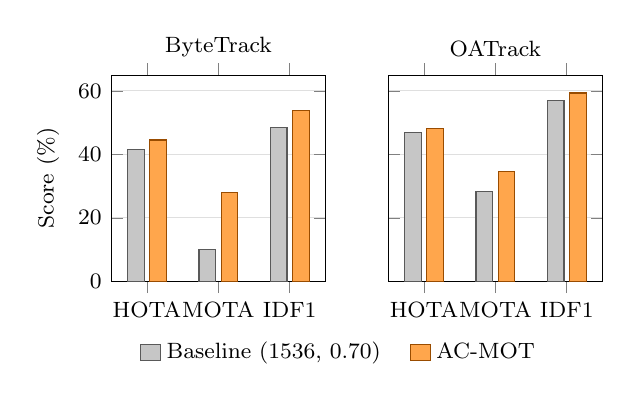
\begin{tikzpicture}
\begin{groupplot}[
  group style={group size=2 by 1, horizontal sep=8mm},
  width=43mm, height=42mm,
  ybar, /pgf/bar width=6pt, ymin=0, ymax=65,
  symbolic x coords={HOTA,MOTA,IDF1}, xtick=data,
  enlarge x limits=0.25,
  ymajorgrids, grid style={gray!25},
  tick label style={font=\footnotesize},
  title style={font=\footnotesize, yshift=-1mm},
  ylabel style={font=\footnotesize},
  legend style={font=\footnotesize, draw=none, legend columns=2,
                at={(1.07,-0.24)}, anchor=north, /tikz/every even column/.append style={column sep=3mm}},
  legend image code/.code={\draw[#1] (0cm,-0.1cm) rectangle (0.25cm,0.1cm);}]
\nextgroupplot[title={ByteTrack}, ylabel={Score (\%)}]
\addplot[fill=gray!45, draw=gray!70!black] coordinates {(HOTA,41.586) (MOTA,9.876) (IDF1,48.569)};
\addplot[fill=orange!70, draw=orange!60!black] coordinates {(HOTA,44.523) (MOTA,27.871) (IDF1,53.929)};
\legend{{Baseline (1536, 0.70)}, {AC-MOT}}
\nextgroupplot[title={OATrack}, yticklabels={}]
\addplot[fill=gray!45, draw=gray!70!black] coordinates {(HOTA,46.770) (MOTA,28.165) (IDF1,57.107)};
\addplot[fill=orange!70, draw=orange!60!black] coordinates {(HOTA,48.095) (MOTA,34.483) (IDF1,59.364)};
\end{groupplot}
\end{tikzpicture}
\caption{HOTA, MOTA, and IDF1 on the seven VisDrone sequences for both
tracker hosts (values in Table~\ref{tab:visdrone}).}
\label{fig:visdrone}
\end{figure}

\begin{table}[t]
\caption{Paired sequence-level bootstrap on VisDrone: AC-MOT minus baseline,
5000 resamples, seed 42. HOTA, MOTA, IDF1, precision, and recall in points;
IDS, FP, and FN in counts.}
\label{tab:bootstrap}
\centering\footnotesize
\setlength{\tabcolsep}{4pt}
\begin{tabular}{@{}llrr@{}}
\toprule
Host & Metric & Difference & 95\% interval\\
\midrule
ByteTrack & HOTA & $+2.937$ & $[+2.356, +3.375]$\\
 & MOTA & $+17.995$ & $[+13.541, +23.282]$\\
 & IDF1 & $+5.360$ & $[+4.490, +6.178]$\\
 & IDS & $-325$ & $[-498, -164]$\\
 & FP & $-14382$ & $[-19176, -9620]$\\
 & FN & $+1781$ & $[+288, +3594.075]$\\
 & Precision & $+10.003$ & $[+8.712, +11.895]$\\
 & Recall & $-2.479$ & $[-4.507, -0.469]$\\
\midrule
OATrack & HOTA & $+1.325$ & $[+0.200, +2.264]$\\
 & MOTA & $+6.318$ & $[+4.741, +7.879]$\\
 & IDF1 & $+2.258$ & $[+0.548, +3.474]$\\
 & IDS & $-169$ & $[-292, -42]$\\
 & FP & $-3994$ & $[-6190, -2494.900]$\\
 & FN & $-375$ & $[-1462.575, +670]$\\
 & Precision & $+3.981$ & $[+2.957, +5.511]$\\
 & Recall & $+0.522$ & $[-0.869, +2.111]$\\
\bottomrule
\end{tabular}
\end{table}

\emph{Paired bootstrap.} Table~\ref{tab:bootstrap} gives the paired differences (AC-MOT minus baseline)
and their 95\% intervals. With ByteTrack, the intervals of HOTA, MOTA, IDF1,
precision, IDS, and FP lie entirely on the side of improvement, and FN and
recall move in the opposite direction. With OATrack, HOTA, MOTA, IDF1, and
precision rise and IDS and FP fall, all with intervals on one side of zero.

\emph{Controller behaviour.} The controller uses all three states with both hosts. With ByteTrack, LOW,
MEDIUM, and HIGH cover 7.4\%, 30.1\%, and 62.5\% of the frames; with OATrack
they cover 7.4\%, 33.3\%, and 59.3\%. The two hosts diverge through their
different tracked boxes. State changes are rare, between 0.10 and 0.54 per 100
frames depending on the sequence, so the detector input stays stable over
long stretches of video.

\subsection{Frozen UAVDT transfer}
The UAVDT transfer uses 20 test sequences with 16,592 frames, scored with one
vehicle class. The frozen controller, thresholds, and action map are applied
without any change. Detector outputs for UAVDT were produced at the three
frozen operating points, giving 49,776 detector forward passes. UAVDT is a
single frozen run per host. The paired bootstrap draws 20 sequences with
replacement from these runs. It is computed from the stored per-sequence
counts of the two systems and therefore covers the count-based metrics MOTA,
IDF1, IDS, FP, and FN.

\begin{table}[t]
\caption{Frozen UAVDT transfer without retuning (20 sequences, 16,592 frames,
one vehicle class). Baseline: fixed operating point (1536, 0.70).}
\label{tab:uavdt}
\centering\footnotesize
\setlength{\tabcolsep}{4pt}
\begin{tabular}{@{}lrrrr@{}}
\toprule
 & \multicolumn{2}{c}{ByteTrack} & \multicolumn{2}{c}{OATrack}\\
\cmidrule(lr){2-3}\cmidrule(l){4-5}
Metric & Baseline & AC-MOT & Baseline & AC-MOT\\
\midrule
HOTA & 45.923 & 47.004 & 47.728 & 47.640\\
MOTA & $-1.573$ & 16.028 & 19.607 & 22.873\\
IDF1 & 58.400 & 61.767 & 62.101 & 62.931\\
IDS & 601 & 486 & 517 & 486\\
FP & 279616 & 212077 & 197937 & 183669\\
FN & 66050 & 73702 & 75612 & 78774\\
Precision & 49.571 & 55.751 & 57.270 & 58.800\\
Recall & 80.625 & 78.381 & 77.820 & 76.893\\
\bottomrule
\end{tabular}
\end{table}

\begin{table}[t]
\caption{Paired sequence-level bootstrap on UAVDT: AC-MOT minus baseline,
5000 resamples, seed 42, 20 sequences. MOTA and IDF1 in points; IDS, FP, and
FN in counts.}
\label{tab:uavdt-boot}
\centering\footnotesize
\setlength{\tabcolsep}{4pt}
\begin{tabular}{@{}llrr@{}}
\toprule
Host & Metric & Difference & 95\% interval\\
\midrule
ByteTrack & MOTA & $+17.601$ & $[+11.134, +26.767]$\\
 & IDF1 & $+3.367$ & $[+1.676, +5.013]$\\
 & IDS & $-115$ & $[-211.025, -26.975]$\\
 & FP & $-67539$ & $[-104215.350, -37352.950]$\\
 & FN & $+7652$ & $[+1542.925, +18359.400]$\\
\midrule
OATrack & MOTA & $+3.267$ & $[+0.607, +5.881]$\\
 & IDF1 & $+0.831$ & $[+0.125, +1.271]$\\
 & IDS & $-31$ & $[-101, +39]$\\
 & FP & $-14268$ & $[-33958.075, -2188.950]$\\
 & FN & $+3162$ & $[-211.100, +8959.050]$\\
\bottomrule
\end{tabular}
\end{table}

Table~\ref{tab:uavdt} and Fig.~\ref{fig:uavdt} report the transfer to UAVDT
without retuning. With ByteTrack, HOTA changes from 45.923 to 47.004 ($+1.081$),
MOTA from $-1.573$ to 16.028 ($+17.601$), and IDF1 from 58.400 to 61.767
($+3.367$). IDS fall by 115 and FP by 67539, while FN rise by 7652. With
OATrack, MOTA changes from 19.607 to 22.873 ($+3.267$), IDF1 from 62.101 to
62.931 ($+0.831$), IDS fall by 31, and FP fall by 14268. With both hosts the
transfer gives fewer FP and IDS and higher precision, with slightly lower
recall, the same pattern as with ByteTrack on VisDrone.

Table~\ref{tab:uavdt-boot} gives the paired bootstrap differences on UAVDT.
With ByteTrack, the intervals of MOTA, IDF1, IDS, and FP lie entirely on the
side of improvement, and FN moves in the opposite direction. With OATrack,
MOTA and IDF1 rise and FP fall, with intervals on one side of zero, while the
intervals of IDS and FN include zero.

\begin{figure}[t]
\centering
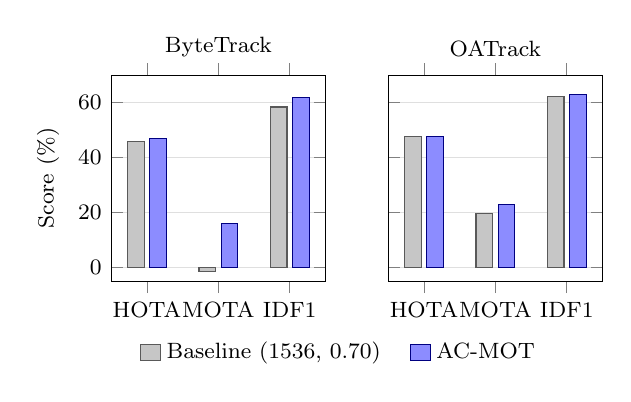
\begin{tikzpicture}
\begin{groupplot}[
  group style={group size=2 by 1, horizontal sep=8mm},
  width=43mm, height=42mm,
  ybar, /pgf/bar width=6pt, ymin=-5, ymax=70,
  symbolic x coords={HOTA,MOTA,IDF1}, xtick=data,
  enlarge x limits=0.25,
  ymajorgrids, grid style={gray!25},
  tick label style={font=\footnotesize},
  title style={font=\footnotesize, yshift=-1mm},
  ylabel style={font=\footnotesize},
  legend style={font=\footnotesize, draw=none, legend columns=2,
                at={(1.07,-0.24)}, anchor=north, /tikz/every even column/.append style={column sep=3mm}},
  legend image code/.code={\draw[#1] (0cm,-0.1cm) rectangle (0.25cm,0.1cm);}]
\nextgroupplot[title={ByteTrack}, ylabel={Score (\%)}]
\addplot[fill=gray!45, draw=gray!70!black] coordinates {(HOTA,45.923) (MOTA,-1.573) (IDF1,58.400)};
\addplot[fill=blue!45, draw=blue!50!black] coordinates {(HOTA,47.004) (MOTA,16.028) (IDF1,61.767)};
\legend{{Baseline (1536, 0.70)}, {AC-MOT}}
\nextgroupplot[title={OATrack}, yticklabels={}]
\addplot[fill=gray!45, draw=gray!70!black] coordinates {(HOTA,47.728) (MOTA,19.607) (IDF1,62.101)};
\addplot[fill=blue!45, draw=blue!50!black] coordinates {(HOTA,47.640) (MOTA,22.873) (IDF1,62.931)};
\end{groupplot}
\end{tikzpicture}
\caption{HOTA, MOTA, and IDF1 of the frozen UAVDT transfer for both tracker
hosts (values in Table~\ref{tab:uavdt}).}
\label{fig:uavdt}
\end{figure}
\section{Discussion}\label{sec:discussion}

\emph{The operating point is part of the MOT system.} The same frozen detector
and the same trackers give very different MOT results at different operating
points. Moving away from the fixed 1536/0.70 point raises MOTA by 17.995 points
with ByteTrack and by 6.318 points with OATrack on VisDrone. The detector
operating point is therefore a first-order variable of aerial MOT and deserves
the same attention as the association method.

\emph{Selective observation streams.} The main effect of AC-MOT is a more
selective detection stream. FP and IDS drop sharply, precision rises, and FN
rise a little with ByteTrack. MOTA reacts most strongly because it counts FP
directly; HOTA and IDF1 rise by smaller amounts. The same pattern appears on
UAVDT, where FP fall by 67539 with ByteTrack and by 14268 with OATrack.

\emph{Tracker dependence.} ByteTrack gains more than OATrack. ByteTrack starts
from a weaker baseline and uses low-score boxes in its second association
step, so a likely reason is that removing clutter helps it directly. OATrack
already weights detections by quality inside its association, and it gains
mainly in MOTA, IDF1, IDS, and FP. Results are therefore reported per host.

\emph{Development path.} The historical profiles showed that the preferred
operating point depends on the goal: quality or identity stability and speed.
The modern stage kept a finite, readable controller with one crowd index, a few
guard cues, three states, and three actions.

\emph{Deployment.} AC-MOT needs no training and no access to detector or
tracker internals. It changes three arguments of the detector call. Its
analysis runs on a quarter-scale image every ten frames and uses boxes that
the tracker already produced. On a Tesla T4 the controller takes 4.26 ms per
frame with ByteTrack and 4.20 ms with OATrack, which is small next to detector
inference. The control layer therefore adds very little latency and is
suitable for real-time use. The same interface can host other action maps, for
example maps chosen for a latency budget, without changes to the detector or
the tracker.
\section{Conclusion}\label{sec:conclusion}

This paper presented Adaptive Control for Multi-Object Tracking (AC-MOT), a
training-free method that automatically adjusts detector settings to improve
multi-object tracking in videos captured by unmanned aerial vehicles (UAVs).
Unlike traditional tracking systems that use fixed detector settings, AC-MOT
changes the detection confidence threshold, non-maximum suppression (NMS) IoU
threshold, and input resolution based on changes in the scene. The method uses
only the current video frame and previous tracking results, without changing
or retraining the detector or tracker. It uses a scene complexity index based
on object density, together with other scene features such as small objects,
illumination, blur, and edges. A three-state controller, supported by
recovery, hysteresis, and dwell-time rules, helps the system adjust its
settings smoothly and avoid frequent changes.

The controller was developed through several optimization experiments to study
how different detector settings affect tracking accuracy, object identity, and
processing time. The results showed that the best detector settings depend on
the tracking method and the performance goal. The final controller settings
were selected using sequence-level cross-validation on separate calibration
videos and were then kept fixed during testing.

Experiments on seven VisDrone2019-MOT video sequences showed that AC-MOT
improved Higher Order Tracking Accuracy (HOTA) by 2.937 points with ByteTrack
and 1.325 points with OATrack. Multiple Object Tracking Accuracy (MOTA) also
increased by 17.995 and 6.318 points, respectively. Paired bootstrap analysis
was used to calculate confidence intervals for the performance differences.
The same controller was also tested on the UAVDT dataset without changing its
settings, improving MOTA by 17.601 points with ByteTrack and 3.267 points with
OATrack.

Overall, the results show that adjusting detector settings during video
processing can improve aerial multi-object tracking without changing the
detector or tracker. They also show that detector settings should be
considered an important part of the tracking system rather than fixed values
used for all video frames. Future work will focus on improving the controller
and testing it with more detectors, tracking methods, and aerial video
datasets.

\backmatter

\section*{Declarations}

\noindent\textbf{Funding.} This research received no external funding.

\noindent\textbf{Conflict of interest.} The authors declare no competing interests.

\noindent\textbf{Ethics approval and consent to participate.} This computational study uses public benchmark data and does not involve human participants or animals.

\noindent\textbf{Consent for publication.} Not applicable.

\noindent\textbf{Data and code availability.} The frozen controller specification, result records, evidence map, staged sections, scripts, and build package are included in the project repository. Dataset redistribution remains subject to the original benchmark licenses and access terms.

\noindent\textbf{Author contributions.} Ahmed Gouda Ismail: Conceptualization, Methodology, Software, Investigation, Data curation, Formal analysis, Visualization, Writing~--~original draft, Writing~--~review \& editing. Mohamed S. Mohamed: Supervision, Methodology, Writing~--~review \& editing. Tarek Ahmed Mahmoud: Supervision, Validation, Writing~--~review \& editing.

\noindent\textbf{Acknowledgements.} Not applicable.

\noindent\textbf{Submission exclusivity.} The manuscript is not under consideration elsewhere and has not been published previously.

\noindent\textbf{AI use in manuscript preparation.} Generative AI tools were used to assist with drafting and language editing. The authors reviewed and verified all content, numerical values, and figures and take full responsibility for the manuscript.

\bibliography{references}

\end{document}
